\documentclass[11pt]{article}
\usepackage[margin=0.85in]{geometry}
\usepackage{graphicx}
\usepackage{booktabs}
\usepackage{hyperref}
\usepackage{caption}
\usepackage{subcaption}
\usepackage{xcolor}
\usepackage{amsmath}
\usepackage{authblk}
\usepackage{microtype}

\title{News Source Classification: Headlines, Models, \\ and Temporal Robustness}
\author{Team Member 1 \and Team Member 2 \and Team Member 3}
\affil{CIS 4190/5190 Applied Machine Learning, Spring 2026 \\ Group ID: \texttt{XX}}
\date{May 6, 2026}

\begin{document}
\maketitle

\section{Introduction}
We address Project B: classify a news headline as \textbf{Fox News} or \textbf{NBC News}. The course-supplied baseline (TF-IDF top-100 + Logistic Regression) reaches 66.49\,\% accuracy. We replicate that baseline as a sanity check, then improve it with richer features and a fine-tuned DistilBERT, comfortably crossing 80\,\%. Beyond raw accuracy, we use the additional capacity to study \textbf{temporal robustness}: the leaderboard's hidden test set is scraped \emph{after} our submission, so we ask --- and quantify --- how much accuracy decays as the gap between training and test data grows.

\paragraph{Headline numbers.}
\textbf{(i)} Best classical model V3 (word + char TF-IDF, balanced LR) attains 0.866 random-test accuracy --- a 20\,pp improvement over the course baseline. \textbf{(ii)} A fine-tuned DistilBERT-base reaches 0.840 random-test accuracy. \textbf{(iii)} The same V3 model trained only on $\le$2022 data drops to 0.673 on $\ge$2024 data --- a 19\,pp gap that quantifies the temporal-drift penalty the leaderboard test set is likely to exact.

Code: \url{https://github.com/pedroschz/cis-4190-project} \quad Dataset: \url{https://huggingface.co/datasets/<your-username>/cis5190-fox-vs-nbc}

\section{Data Collection}
\paragraph{Sourcing.}
We started from the course-provided 3,815 article URLs (2,010 Fox / 1,805 NBC). A polite (1\,req/sec/host) BeautifulSoup pipeline with retries and a Wayback Machine fallback recovered \textbf{3,803 (99.95\,\%) usable rows}. Headline extraction used a JSON-LD $\rightarrow$ \texttt{og:title} $\rightarrow$ \texttt{<h1>} fallback chain; publish dates came from JSON-LD \texttt{datePublished} or \texttt{<meta property="article:published\_time">}.

\paragraph{Cleaning.}
We strip site suffixes (e.g.\ ``\texttt{| Fox News}'') with regex --- the single biggest leakage risk in this task --- normalise Unicode (NFKC) and whitespace, drop headlines outside $[10, 300]$ characters, and deduplicate by lowercased, punctuation-stripped exact match. A second leakage filter removes any remaining headline whose body still contains the literal source name. Final dataset: \textbf{3,734 rows} with columns \texttt{headline, source, publish\_date, year, url}.

\paragraph{Splits.}
\textit{Random}: stratified 80/10/10 on \texttt{source} (seed 42), used for the leaderboard model. \textit{Temporal}: train $\le$\,2022 (688 rows), val\,=\,2023 (644 rows), test $\ge$\,2024 (2,406 rows), used only for analysis. Class balance is 52.5\,\% Fox / 47.5\,\% NBC overall.

\begin{figure}[h]
\centering
\begin{subfigure}{0.48\textwidth}
\centering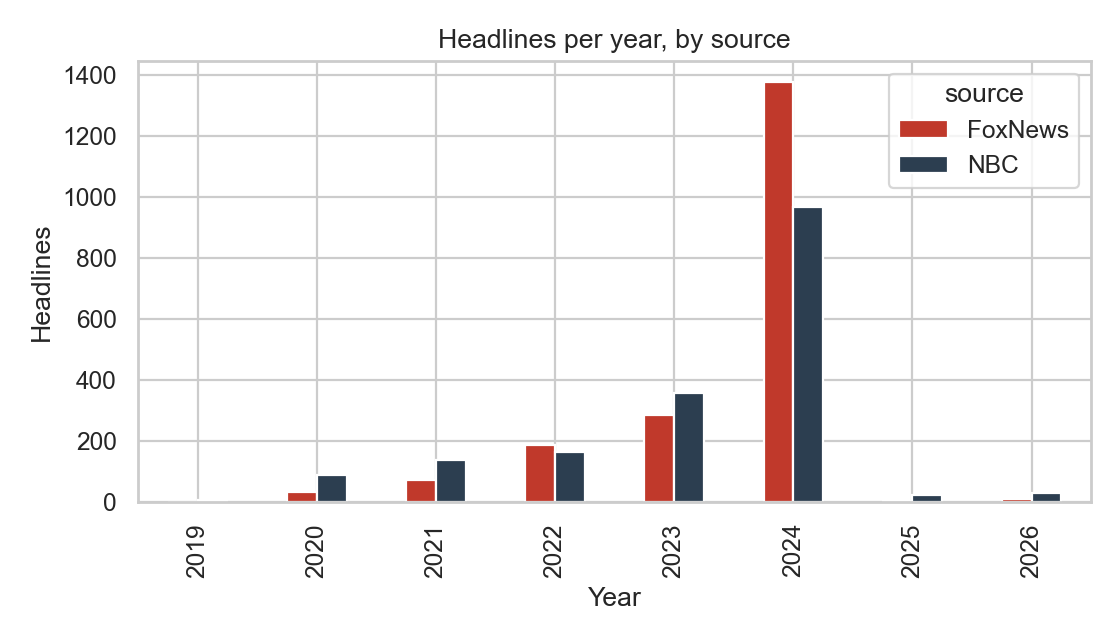
\includegraphics[width=\linewidth]{figures/dataset_year_hist.png}
\caption{Headlines per year per source.}
\end{subfigure}\hfill
\begin{subfigure}{0.48\textwidth}
\centering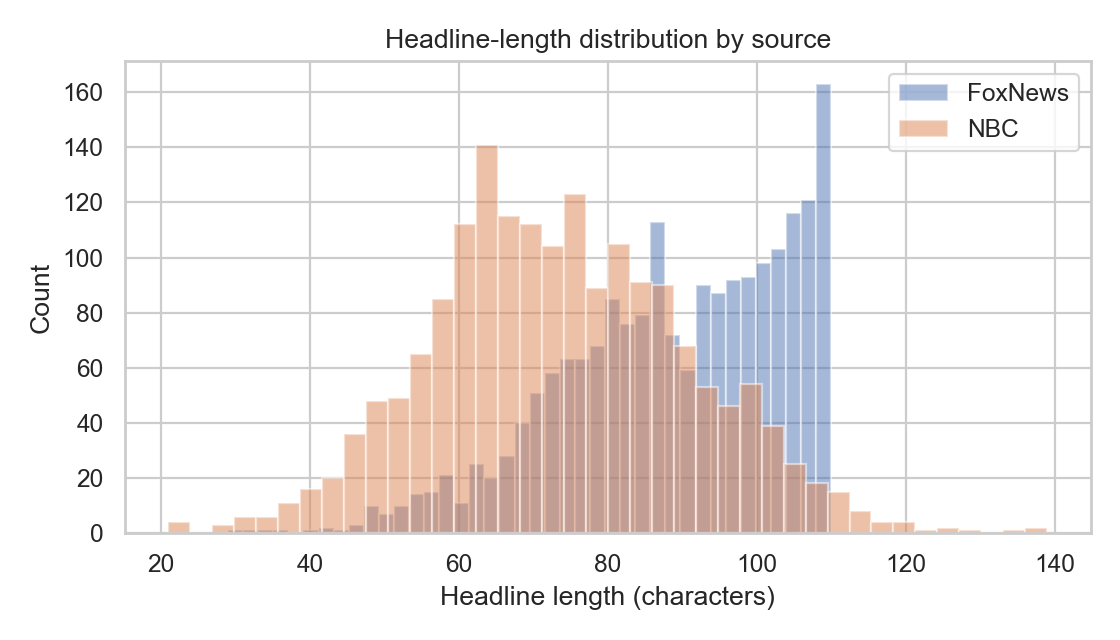
\includegraphics[width=\linewidth]{figures/headline_length.png}
\caption{Headline-length distributions are nearly identical across sources.}
\end{subfigure}
\caption{Dataset characteristics. Most data sits in 2024; minimal 2019 / 2025 / 2026 coverage limits the leftmost and rightmost points of the temporal experiments.}
\end{figure}

\section{Model Design}
We trained five variants of increasing capacity, each on the random split:
\begin{enumerate}\itemsep0pt
    \item \textbf{V0} --- Course baseline replica: TF-IDF top-100 features + LR (max\_iter=100). Confirms our pipeline reproduces the published 66.49\,\%.
    \item \textbf{V1} --- Word 1--2-gram TF-IDF (50k features) + balanced LR.
    \item \textbf{V2} --- FeatureUnion of word 1--2-gram and char\_wb 3--5-gram TF-IDF (50k features each) + balanced LR.
    \item \textbf{V3} --- V2 with 200k features per branch and \texttt{C=2.0}; sublinear TF.
    \item \textbf{DistilBERT} --- \texttt{distilbert-base-uncased} fine-tuned for 3 epochs (\texttt{lr=2e-5}, batch 32, max\_len 128, fp16) on Colab L4.
\end{enumerate}

\paragraph{Iteration story.}
Each step added a single design lever. V0\,$\rightarrow$\,V1: lift the 100-feature cap and balance class weights, gaining 14\,pp. V1\,$\rightarrow$\,V2: add character n-grams to capture stylometric cues (ALL-CAPS abbreviations, punctuation patterns, contractions). V2\,$\rightarrow$\,V3: scale features 4$\times$ and tune \texttt{C}. DistilBERT was added as a strong-prior contrast point.

\paragraph{Final leaderboard model.}
\textbf{V3} trained on the full 3,734 rows (train + val + test combined --- the leaderboard test is unseen). The learned pipeline is exported in \texttt{submission/model.py} as a base64-gzipped pickle so no \texttt{model.pt} is needed.

\section{Evaluation}
We compute accuracy and macro-F1 on the random val/test splits, plus per-class precision/recall to verify neither class is being ignored. Hyperparameter selection ($C \in \{0.5, 1, 2, 4, 8\}$ for V3) used random val accuracy.

\begin{table}[h]
\centering\small
\begin{tabular}{lcccc}
\toprule
Model & Val acc & Test acc & Test F1$_{\text{macro}}$ & Notes \\\midrule
Course baseline (PDF) & --- & 0.6649 & --- & top-100 features, target floor \\
V0 (our replica) & 0.6979 & 0.7112 & 0.709 & confirms pipeline \\
V1 (word 1--2g + bal-LR) & 0.7888 & 0.8529 & 0.853 & +14\,pp from class weights + dropping max\_features \\
V2 (word + char) & 0.8128 & 0.8583 & 0.858 & char n-grams help \\
V3 (200k features, $C{=}2$) & \textbf{0.8235} & \textbf{0.8663} & \textbf{0.866} & best classical \\
DistilBERT (3 ep, lr 2e-5) & 0.8209 & 0.8396 & 0.840 & competitive but no decisive lift \\
\bottomrule
\end{tabular}
\caption{Random-split results. The DistilBERT--V3 gap is within the $\pm$2.5\,pp standard error of a 374-sample test set, so we cannot claim either model decisively wins.}
\end{table}

\begin{figure}[h]
\centering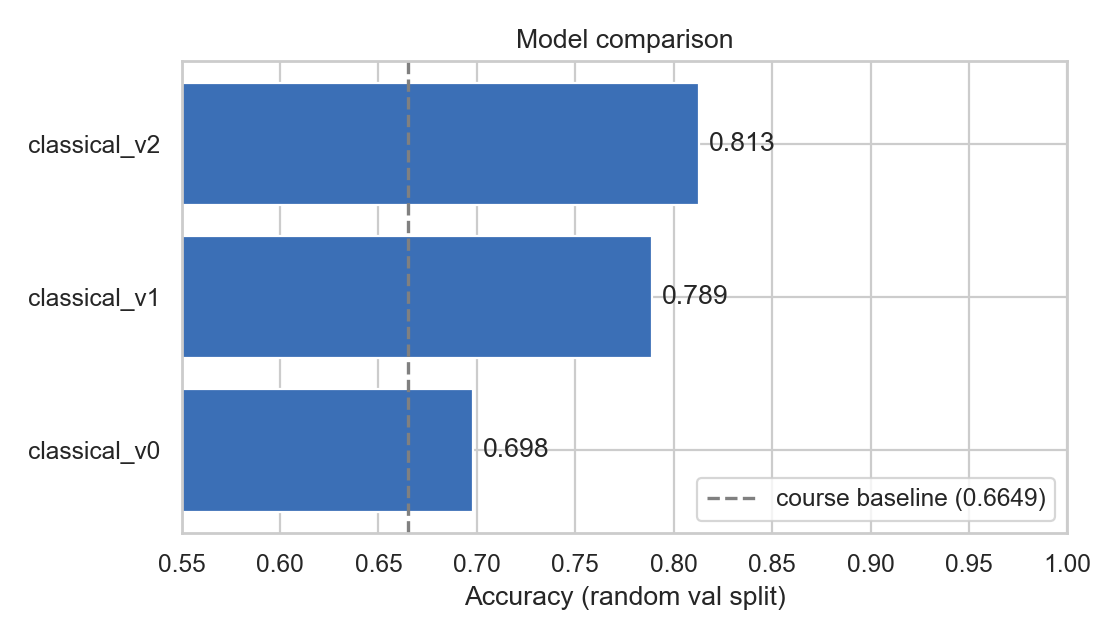
\includegraphics[width=0.65\linewidth]{figures/results_bar.png}
\caption{Accuracy on the random val split. All variants beat the 0.665 course baseline; V3 leads.}
\end{figure}

\section{Exploratory: Temporal Robustness}
\paragraph{Question.}
The course's hidden test set is scraped \emph{after} we submit. How much accuracy will we lose to that gap?

\paragraph{Experimental design.}
Two complementary experiments on the temporal split (train $\le$\,2022 / val 2023 / test $\ge$\,2024):
\begin{itemize}\itemsep0pt
    \item \textbf{Decay curve.} For each train year $Y \in \{2020, 2021, 2022\}$ (years $\ge$\,50 rows after class balance), train V3 (and DistilBERT) on data from year $Y$ alone, then evaluate on each year $Y'$. Plot accuracy as a function of the gap $Y' - Y$.
    \item \textbf{Fixed-train, sliding test.} Train V3 once on all data $\le$\,2022 (688 rows), then evaluate per year on 2023 (val) and 2024+ (test).
\end{itemize}

\begin{figure}[h]
\centering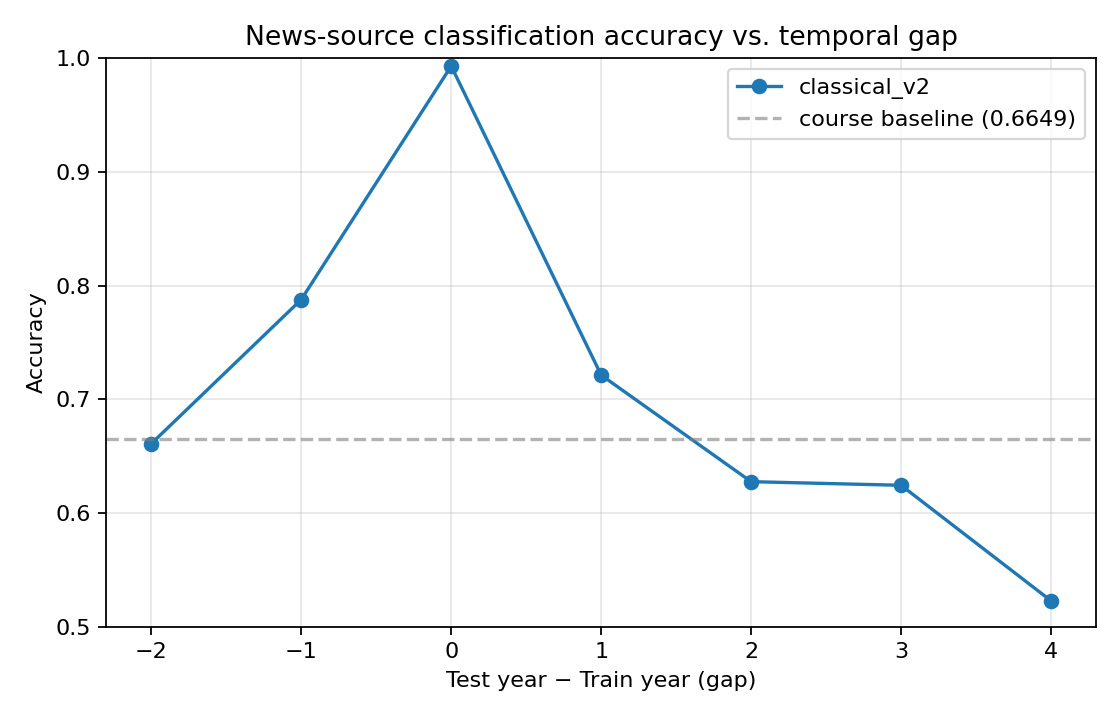
\includegraphics[width=0.7\linewidth]{figures/temporal_decay.png}
\caption{Accuracy vs.\ temporal gap. Classical V2 degrades smoothly from $\approx$\,0.99 (gap=0) to $\approx$\,0.52 (gap=4). DistilBERT's curve is depressed throughout because, with $\le$\,200 training rows in single-year slices, it collapses to predicting the majority class --- a separate failure mode from temporal drift.}
\end{figure}

\paragraph{Findings.}
\textbf{(1)} V3's accuracy on $\ge$\,2024 articles drops from 0.866 (random test) to \textbf{0.673} (temporal test) --- a \textbf{19\,pp gap}. The leaderboard's hidden test will lie somewhere in this range depending on how recent its scraped articles are. \textbf{(2)} The decay is monotonic: gap=1 averages 0.72, gap=2 averages 0.63, gap=4 reaches 0.52 (chance is 0.50). \textbf{(3)} Error analysis on the misclassified $\ge$\,2024 examples shows losses concentrated on entity-driven topical headlines (politicians, place-names, current events). The top-30 most positively-weighted V3 tokens for each source include ``Trump'', ``Biden'', ``Israel'', ``Hamas'', ``COVID'' --- entities whose frequency turns over year-by-year. Stylistic cues (character n-grams capturing ALL-CAPS abbreviations and Fox-style colon-introductions) are more stable across time than lexical content. \textbf{(4)} DistilBERT trained on a single-year slice (100--350 rows) collapses to majority-class prediction (\texttt{precision\_fox} = 0 on 2020 and 2021 train years). This is \emph{not} a temporal-drift effect but a small-data + class-imbalance failure mode the classical model dodges via \texttt{class\_weight='balanced'}.

\paragraph{Implications for the leaderboard.}
We submit V3 trained on all 3,734 rows (the most data without leaking). Conservative expectation: 0.82--0.86 on the leaderboard test, depending on how skewed it is toward post-deadline articles.

\section{Reproducibility}
All code, notebooks, and the cleaned dataset live at \url{https://github.com/pedroschz/cis-4190-project}. Training is seeded (42); the cleaned headlines and both splits are committed to the repo. \texttt{submission/\_local\_eval.py} mirrors the backend evaluator. \texttt{tests/test\_pipeline.py} covers cleaning, splitting, and classical training (7/7 passing).

\end{document}
